\section{Datasets and analysis}
\begin{table}
    \centering
    \caption{Datasets used in definition modeling}
    \begin{tabular}{|ll|}
        \hline
        Dataset          & Methods                              \\
        \hline
        Oxford & \cite{bevilacqua_generationary_2020,
        chang_what_2019,
        gadetsky_conditional_2018,
        ishiwatari_learning_2019,
        li_explicit_2020,
        mickus_mark_2019,
        reid_vcdm_2020,
        washio_bridging_2019} \\
        WordNet & \cite{bevilacqua_generationary_2020,
        ishiwatari_learning_2019,
        kabiri_evaluating_2020,
        li_explicit_2020,
        mickus_mark_2019,
        noraset_definition_2016,
        washio_bridging_2019} \\
        Urban Dictionary & \cite{reid_vcdm_2020,
        ishiwatari_learning_2019,
        ni_learning_2017}\\
        Wikipedia & \cite{huang_cdm_2021,
        reid_vcdm_2020}\\
        Wiktionary & \cite{bevilacqua_generationary_2020,
        kabiri_evaluating_2020}\\
        OmegaWiki & \cite{kabiri_evaluating_2020}\\
        Hei++ & \cite{bevilacqua_generationary_2020}\\
        \hline
    \end{tabular}
    \label{tab:eval}
\end{table}

Various benchmark datasets have been proposed for the training and evaluation of
definition models. In this section, we provide brief descriptions of each
dataset and provide analysis of various characteristics of the datasets.

\textbf{Oxford Dictionary:}
\textit{The Oxford Dictionary of
    English}\footnote{\href{https://languages.oup.com/}{https://languages.oup.com/}}
is a free dictionary of English words and phrases. Collected by Gadetsky et
al., this dataset features contextual information for each word along with
the definition \cite{gadetsky_conditional_2018}. This dataset is useful for
evaluating the ability of a model to generate definitions for polysemous
words.

\textbf{GCIDE/WordNet:}
\textit{The GNU Collaborative International Dictionary of
    English}\footnote{\href{https://gcide.gnu.org.ua/}{https://gcide.gnu.org.ua/}}
(GCIDE) is a free dictionary supplemented with some definitions from
WordNet\footnote{\href{https://wordnet.princeton.edu/}{https://wordnet.princeton.edu/}}.
Available under the GNU General Public License, GCIDE is a useful corpus for
dictionary definitions for general words. This dataset was modified by
Noraset et al. for their original definition model
\cite{noraset_definition_2016}. Kabiri et al. also provide a modified
dataset for their method \cite{kabiri_evaluating_2020}.

\textbf{Urban Dictionary:}
\textit{The Urban
    Dictionary}\footnote{\href{https://www.urbandictionary.com/}{https://www.urbandictionary.com/}}
is a free dictionary of slang words and phrases where definitions are
crowd-sourced by users. Proposed by Ni et al., the Urban Dictionary dataset
is useful for idioms and rarely-used phrases which are not contained in
other dictionary datasets due to only containing slang definitions
\cite{ni_learning_2017}.

\textbf{Wikipedia:}
\textit{The English
    Wikipedia}\footnote{\href{https://en.wikipedia.org/}{https://en.wikipedia.org/}}
is a free online encyclopedia. Collected by Ishiwatari et al., it combines
the useful tasks of WordNet, Oxford Dictionary, and Urban Dictionary, since
it contains descriptions of many concepts along with context to be used in
context-aware models \cite{ishiwatari_learning_2019}.

\textbf{Wiktionary:}
\textit{Wiktionary}\footnote{\href{https://en.wiktionary.org/}{https://en.wiktionary.org/}}
is a free online dictionary from the same parent organization as Wikipedia
(Wikimedia Foundation). It is useful as it provides a definitions for a large
number of languages which can allow for multi-lingual definition modeling. We
share statistics for the English version of Wiktionary, since most definition
modeling methods focus on English.

\textbf{OmegaWiki:}
Similar to Wiktionary, \textit{OmegaWiki} is a multi-lingual dictionary. The
goal of OmegaWiki is to create a lexical resource with all definitions of all
words in every language. Kabiri et al. use this resource due to the availability
of a variety of languages \cite{kabiri_evaluating_2020}.

\textbf{Hei++:}
\textit{Hei++}\footnote{\href{http://generationary.org/}{http://generationary.org/}}
is a unique evaluation dataset proposed by Bevilacqua et al.
\cite{bevilacqua_generationary_2020}. Rather than contain singular words or
phrases to define like the other dictionary-based resources, this dataset is
comprised of adjective-noun phrases. An example phrase, \textit{starry sky}, can
be defined as 'The sky as it appears at night, especially when lit by stars'.
This is a hand-made dataset which was create with the assistance of an expert
lexicographer. As a result, this dataset is small and should be used in model
evaluation rather than training. Our dataset analysis shows no overlap of this
dataset with the other benchmark datasets, implying this dataset can also be
used to evaluating the ability of a model to generalize on never-before-seen
data.

\subsection{Definition Statistics}

In our analysis of the datasets above, to distinguish the benchmark datasets
provided by the correlating authors, we use the notations listed in Table
\ref{tab:ds_notations}.

\begin{table}[h]
    \centering
    \caption{Dataset notations}
    \begin{tabular}{|l|l|}
    \hline
    Dataset                  & Description                                                                                     \\
    \hline
    \textit{wordnet-nor}     & WordNet dataset, from Noraset et al. \cite{noraset_definition_2016}                             \\
    \textit{urban-ni}        & Urban Dictionary dataset, from Ni et al. \cite{ni_learning_2017}                                \\
    \textit{oxford-gad}      & The Oxford Dictionary of English dataset, from Gadetsky et al. \cite{gadetsky_conditional_2018} \\
    \textit{wordnet-ish}     & WordNet dataset, from Ishiwatari et al. \cite{ishiwatari_learning_2019}                         \\
    \textit{wikipedia-ish}   & Wikipedia dataset, from Ishiwatari et al. \cite{ishiwatari_learning_2019}                       \\
    \textit{wikitionary-kab} & Wikitonary English dataset, from Kabiri et al. \cite{kabiri_evaluating_2020}                    \\
    \textit{wordnet-kab}     & WordNet dataset, from Kabiri et al. \cite{kabiri_evaluating_2020}                               \\
    \textit{omega-kab}       & OmegaWiki dataset, from Kabiri et al. \cite{kabiri_evaluating_2020}                             \\
    \textit{hei++-bev}       & Hei++ dataset, from Bevilacqua et al. \cite{bevilacqua_generationary_2020}                      \\
    \hline
\end{tabular}

    \label{tab:ds_notations}
\end{table}

First, in Table \ref{tab:defs}, we provide some analysis on the definition
statistics of the datasets. We evaluate all splits (train, test, and validate)
for each dataset by combining all the words and corresponding definitions. The
table shows the number of unique words and total number of definitions for each
dataset. Of note, some datasets provide the same definition for the same word,
meant to be used in a context-aware model. In this analysis, we ignore the
context phrases and treat these duplicate definitions as independent. We also
show the mean length of the definitions, the standard deviation of the lengths,
as well as the \textit{definitions per word} (DPW).

\begin{table}
    \centering
    \caption{Definition statistics}
    \begin{tabular}{|l|rr|rrr|}
    \hline
    Dataset        & Words   & Definitions & DPW  & Mean length & SD length \\
    \hline
    wikipedia-ish  & 168,753 & 988,690     & 5.86 & 5.99        & 4.53      \\
    urban-ni       & 240,334 & 507,504     & 2.11 & 12.11       & 7.71      \\
    wordnet-nor    & 22,554  & 162,925     & 7.22 & 6.60        & 5.73      \\
    oxford-gad     & 36,767  & 122,319     & 3.33 & 11.07       & 7.01      \\
    wiktionary-kab & 17,000  & 29,426      & 1.73 & 7.65        & 6.92      \\
    wordnet-kab    & 20,000  & 28,814      & 1.44 & 10.96       & 7.28      \\
    omega-kab      & 17,000  & 22,735      & 1.34 & 14.61       & 9.83      \\
    wordnet-ish    & 9,937   & 17,410      & 1.75 & 6.64        & 3.78      \\
    hei++-bev      & 713     & 713         & 1.00 & 9.44        & 2.80      \\
    \hline
\end{tabular}

    \label{tab:defs}
\end{table}

Next, in Table \ref{tab:polys}, we show the number of polysemous words in each
dataset. As with the definition statistics, we treat exact duplicate definitions
independently, because they have different contexts. The number of polysemes is
calculated as the number of words or phrases which have more than one definition
in the dataset. We show the ratio of the number of polysemous words to the total
number of words in the dataset as a percentage. The polysemous data is also
shown in Figure \ref{fig:polys}.  It is important to evaluate the polysemous
data due to the difficulty in predicting definitions for polysemous words.

\begin{table}
    \centering
    \caption{Polyseme statistics}
    \small
\begin{tabular}{|l|rrr|}
    \hline
    Dataset    & Words   & Polysemes & Polysemes (\%) \\
    \hline
    WordNet-A  & 22,554  & 22,171    & 98             \\
    Oxford     & 36,767  & 20,563    & 56             \\
    Wikipedia  & 168,753 & 77,278    & 46             \\
    WordNet-B  & 9,937   & 4,221     & 42             \\
    Urban      & 240,334 & 74,620    & 31             \\
    Wiktionary & 17,000  & 4,634     & 27             \\
    Omega      & 17,000  & 3,412     & 20             \\
    WordNet-C  & 20,000  & 3,649     & 18             \\
    Hei++      & 713     & 0         & 0              \\
    \hline
\end{tabular}

    \label{tab:polys}
\end{table}

% \begin{figure}
%     \centering
%     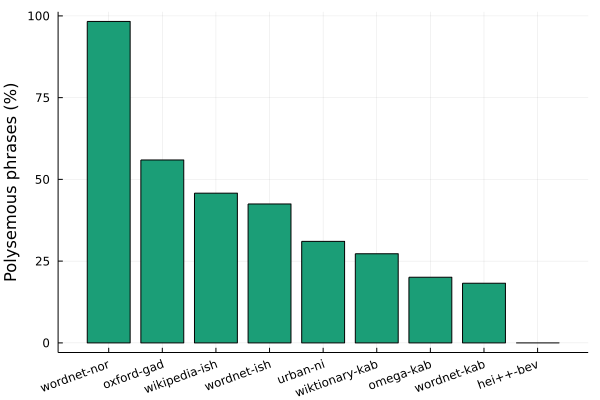
\includegraphics[width=0.65\textwidth]{assets/plots/polys_plot.png}
%     \caption{Plot of polyseme statistics, where the percentage of words or
%         phrases that are polysemous are shown.} \label{fig:polys}
% \end{figure}

Our next analysis is on the overlap present across the benchmark datasets. We
show the number of words in each dataset which are present in all other datasets
as a percentage. This allows us to identify the datasets which are most similar
and most unique. The overlap of each dataset is calculated as the unique words
that are present in each other dataset. The average overlap percentage is shown
in Figure \ref{fig:avg_overlap}, and the individual overlap of each dataset is
shown in Figure \ref{fig:overlap_all}. The Hei++ dataset is not included in the
individual overlap plot due to having an average overlap percentage of $0\%$
\cite{bevilacqua_generationary_2020}. Also, the individual overlap of each
dataset with itself is excluded, as the overlap would be $100\%$.

\begin{figure}
    \centering
    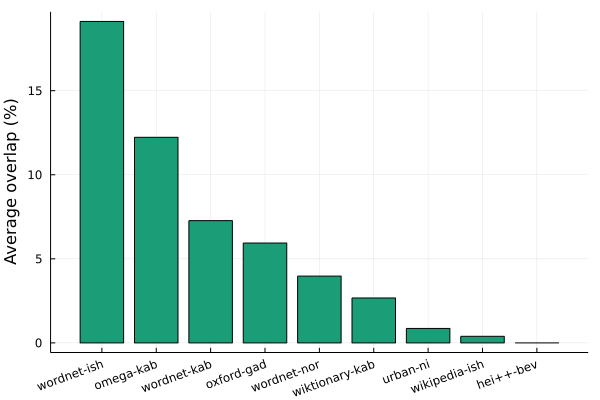
\includegraphics[width=0.7\textwidth]{assets/plots/avg_overlap.png}
    \caption{Plot of average dataset overlap.}
    \label{fig:avg_overlap}
\end{figure}

\begin{figure}
    \centering
    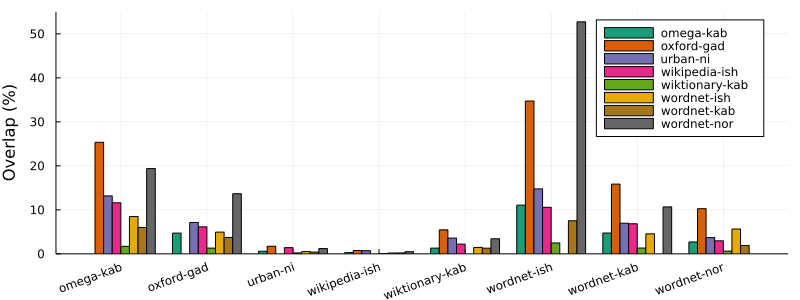
\includegraphics[width=0.95\textwidth]{assets/plots/overlap_all.png}
    \caption{Plot of individual dataset overlap.}
    \label{fig:overlap_all}
\end{figure}

\FloatBarrier
Across every benchmark dataset (excluding Hei++), a single word that is present
in each is the word \textit{movement}. Since it is the only word present in each
dataset, we show selected definitions for this word in Table \ref{tab:movement}. Several different word senses can be seen across the dataset, such as movement as something moving, a specific album, bowel movement, and even the illusion of something moving.

\begin{table}[h]
    \centering
    \caption{Definitions for the term \textit{movement}}
    \begin{tabular}{|l|l|}
    \hline
    Dataset        & Definition                                                                                                                                  \\
    \hline
    wordnet-nor    & \makecell[l]{a natural event that involves a change in the position or location of something}                                                             \\
    \hline
    oxford-gad     & \makecell[l]{a group of people with a common ideology who try together to achieve\\ certain general goals}                                                  \\
    \hline
    wordnet-ish    & a major self-contained part of a symphony or sonata                                                                                         \\
    \hline
    wikipedia-ish  & album by new order                                                                                                                          \\
    \hline
    urban-ni       & [pot credit] slang, to hit on a woman                                                                                                       \\
    \hline
    wordnet-kab    & \makecell[l]{an optical illusion of motion produced by viewing a rapid succession of\\ still pictures of a moving object}                                   \\
    \hline
    wiktionary-kab & the deviation of a pitch from ballistic flight                                                                                              \\
    \hline
    omega-kab      & \makecell[l]{what a dogs body releases from time to time as a little pile of waste\\
                    remaining from digestion , after it has been collected in the colon .} \\
    \hline
\end{tabular}

    \label{tab:movement}
\end{table}

The final analysis is on single word definitions. In most of the datasets, there
are some definitions which consist only of a single word. Single word
definitions may cause evaluation criteria such as BLEU to be difficult to
improve. We show the percentage of definitions in each dataset which consist of
only a single word. We also show the number of single word definitions in each
dataset which are considered to be a synonym of the word or phrase being
defined. We used WordNet synsets in order to identify synonymous words. The
single word definition analysis is shown in Figure \ref{fig:single_word_defs}.

\begin{figure}
    \centering
    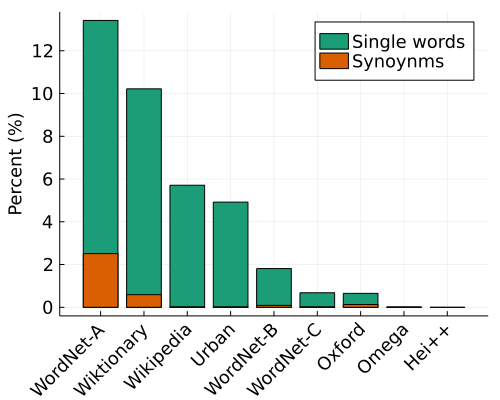
\includegraphics[width=0.7\textwidth]{assets/plots/syn_counts.png}
    \caption{Plot of single word definitions.}
    \label{fig:single_word_defs}
\end{figure}
